%%%%%%%%%%%%%%%%%%%%%%%%%%%%%%%%%%%%%%%%%%%%%%%%%%%%%%%%%%%%%%%%%%%%%%%%%%%%%%%%
%2345678901234567890123456789012345678901234567890123456789012345678901234567890
%        1         2         3         4         5         6         7         8

\documentclass[letterpaper, 10 pt, conference]{ieeeconf}  % Comment this line out if you need a4paper

%\documentclass[a4paper, 10pt, conference]{ieeeconf}      % Use this line for a4 paper

\IEEEoverridecommandlockouts                              % This command is only needed if 
                                                          % you want to use the \thanks command

\overrideIEEEmargins                                      % Needed to meet printer requirements.

% See the \addtolength command later in the file to balance the column lengths
% on the last page of the document

% The following packages can be found on http:\\www.ctan.org
%\usepackage{graphics} % for pdf, bitmapped graphics files
%\usepackage{epsfig} % for postscript graphics files
%\usepackage{mathptmx} % assumes new font selection scheme installed
%\usepackage{times} % assumes new font selection scheme installed
%\usepackage{amsmath} % assumes amsmath package installed
%\usepackage{amssymb}  % assumes amsmath package installed



\usepackage{amsmath,amssymb}

\usepackage{tikz,hyperref,graphicx,units,subfig}
\usepackage{benktools}
\usepackage{caption}
\renewcommand{\captionfont}{\footnotesize}
\usepackage{sidecap,wrapfig}
\usepackage[ruled,vlined]{algorithm2e}
\DeclareMathOperator*{\argmin}{arg\,min}
\DeclareMathOperator*{\argmax}{arg\,max}
\newcommand{\abs}[1]{\lvert#1\rvert} 
\newcommand{\norm}[1]{\lVert#1\rVert}
%\newcommand{\suchthat}{\mid}
\newcommand{\suchthat}{\ \big|\ }
\newcommand{\bd}{\mathbf{d}}
\newcommand{\bn}{\mathbf{n}}
\newcommand{\bp}{\mathbf{p}}
\newcommand{\bw}{\mathbf{w}}
\newcommand{\bt}{\mathbf{t}}
\newcommand{\by}{\mathbf{y}}
\newcommand{\bx}{\mathbf{x}}
\newcommand{\bz}{\mathbf{z}}
\newcommand{\bbf}{\mathbf{f}}
\newcommand{\bzero}{\mathbf{0}}
\newcommand{\bG}{\mathbf{G}}
\newcommand{\bA}{\mathbf{A}}
\newcommand{\bW}{\mathbf{W}}
\newcommand{\bX}{\mathbf{X}}
\newcommand{\mX}{\mathcal{X}}
\newcommand{\mD}{\mathcal{D}}
\newcommand{\mN}{\mathcal{N}}
\newcommand{\mW}{\mathcal{W}}
\newcommand{\mF}{\mathcal{F}}
\newcommand{\bZ}{\mathbf{Z}}

\newcommand{\bfc}{W}
\newcommand{\Qinf}{Q_{\infty}}
\newcommand{\st}[1]{_\text{#1}}
\newcommand{\rres}{r\st{res}}
\newcommand{\pos}[1]{(#1)^+}
\newcommand{\depth}{\operatorname{depth}}
\newcommand{\dist}{\operatorname{dist}}
\newcommand{\convhull}{\operatorname{ConvexHull}}
\newcommand{\minksum}{\operatorname{MinkowskiSum}}

\title{\LARGE \bf
Budgeted Multi-Armed Bandit Models for Sample-Based Grasp Planning in the Presence of Uncertainty}


\author{Michael Laskey$^1$,Jeff Mahler$^1$, Zoe McCarthy$^1$,  Florian T. Pokorny$^3$, Sachin Patil$^1$,\\ Jur Van Den Berg$^4$,  Danica Kragic$^3$, Pieter Abbeel$^1$, Ken Goldberg$^2$% <-this % stops a space
\thanks{$^1$Department of Electrical Engineering and Computer Sciences; {\small \{mdlaskey, zmccarthy, jmahler, sachinpatil, pabbeel\}@berkeley.edu}}%
\thanks{$^2$Department of Industrial Engineering and Operations Research and Department of Electrical Engineering and Computer Sciences; {\small goldberg@berkeley.edu}}%
\thanks{$^{1-2}$ University of California, Berkeley;  Berkeley, CA 94720, USA}%
\thanks{$^3$Computer Vision and Active Perception Lab, Centre for Autonomous Systems, School of Computer Science and Communication, KTH Royal Institute of Technology, Stockholm, Sweden {\small \{fpokorny, dani\}@kth.se}}%
\thanks{$^4$Google; Amphitheatre Parkway, Mountain View, CA 94043, USA {\small jurvandenberg@gmail.com}}%
} 

\newtheorem{theorem}{Theorem}

\begin{document}



\maketitle
\thispagestyle{empty}
\pagestyle{empty}


%%%%%%%%%%%%%%%%%%%%%%%%%%%%%%%%%%%%%%%%%%%%%%%%%%%%%%%%%%%%%%%%%%%%%%%%%%%%%%%%


\begin{abstract}
Sampling perturbations in shape, state, and control can facilitate grasp planning in the presence of uncertainty arising from noise, occlusions, and surface properties such as transparency and specularities.  Monte-Carlo sampling is computationally demanding, even for planar models. We consider an alternative based on the multi-armed bandit (MAB) model for making sequential decisions, which can apply to a variety of uncertainty models.  We formulate grasp planning as a ``budgeted multi-armed bandit model" (BMAB) with finite stopping time to minimize ``simple regret", the difference between the expected quality of the best grasp and the expected quality of the grasp evaluated at the stopping time.  To evaluate MAB-based sampling, we compare it with Monte-Carlo sampling for grasping an uncertain planar object with shape uncertainty defined by a Gaussian process implicit surface (GPIS), but the method is also applicable to other models of uncertainty.  We derive distributions on contact points, surface normal, and center of mass under shape uncertainty and use these to formulate the associated MAB model, finding that it computes grasps of similar quality to Monte-Carlo sampling and can reduce computation time by an order of magnitude.  This suggests a number of new research questions about how MAB can be applied to other models of uncertainty and how different MAB solution techniques can be applied to further reduce computation.
\end{abstract}

%%%%%%%%%%%%%%%%%%%%%%%%%%%%%%%%%%%%%%%%%%%%%%%%%%%%%%%%%%%%%%%%%%%%%%%%%%%%%%%%

\section{Introduction}


%\vspace{10pt}
%\todo{Get High res GPIS visualizations, Incorporate next round of feedback}

Consider a robot packing boxes in a shipping warehouse environment, where it may frequently encounter new consumer products and need to process them quickly.
The robot may need to rapidly plan grasps for these objects without prior knowledge of their shape, pose and material properties like friction coefficient or center of mass. 
Furthermore, the robot may not be able to measure these quantities exactly due to sensor noise and missing data resulting from partial visibility and object properties such as transparency, .
Grasp planners that assume exact prior knowledge of object geometry or an exact measurement of pose may fail in this environment.

Grasp quality metrics have been developed to determine if a grasp will be successful or not and how much force it needs to exert to resist an opposing force, however most of them evaluate a grasp assuming all the parameters are known \cite{ferrari1992}.
Recent work motivated using knowledge of uncertainty to select grasps, but most methods for evaluating grasp quality in the presence of uncertainty requires exhaustive sampling over the possible values of the uncertain quantity \cite{kim2012physically, weisz2012pose}.
To select a grasp with high quality this evaluation must be performed for a large set of potential grasps, which can be very time-consuming.
However, when evaluating a set of grasps we may be able to determine the difference of quality between grasps with only a few samples and throw away grasps that are likely to be suboptimal \cite{kehoe2012estimating}.
Thus, we can adaptively concentrate grasp quality evaluation on the grasps that are most likely to have the highest quality based on the evaluation done so far.

\begin{figure}[t!]
\centering
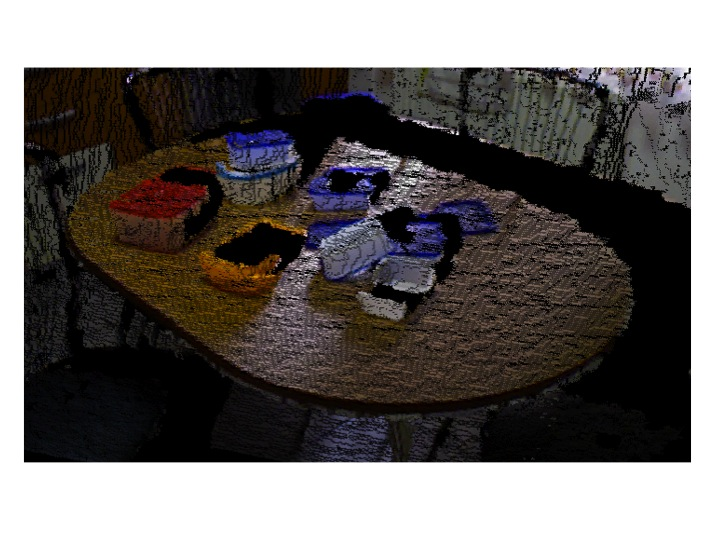
\includegraphics[width=8.5cm,height=8cm]{figures/Slide02.jpg}
\caption{\footnotesize
Convergance in regret of the bandit sampling method (red), compared to the traditional Monte-Carlo method. The fast convergence of the bandit method is due to its ability to intelligently pick what grasp to sample next in a given set of proposed grasps on an object with shape uncertainty}
\vspace*{-10pt}
\label{fig:noisy data}
\end{figure}

The multi-armed bandit (MAB) model for sequential decision making problems \cite{barto1998reinforcement, lai1985asymptotically, robbins1952some} provides a way to reason about selecting the next grasp to evaluate and the grasps to discard from consideration.
The goal in a MAB model is to make a sequence of decisions over a set of possible options, or ``arms", such that a measure of the expected reward of such decisions is maximized.
Solutions to the MAB model are particularly useful in applications where it is too expensive to fully evaluate a set of options; for example, in optimal design of clinical trials~\cite{simon1989optimal}, market pricing~\cite{rothschild1974two}, and choosing strategies for games~\cite{st2012online}.
The budgeted multi-armed bandit model \cite{madani2004budgeted} is a specialization of the MAB model with a finite number of total decisions to be made before a predetermined `stopping time'.
The objective is to maximize the expected reward of the decision made at the stopping time, or equivalently to minimize ``simple regret", which is the difference between the true expected reward of an optimal arm and the true expected reward of the arm pulled at the stopping time.

Our main contribution in this paper is formulating the problem of planning grasps according to some quality metric in the presence of uncertainty as a budgeted multi-armed bandit model.
We use this formulation to rank a set of potential grasps by the probability of force closure \cite{christopoulos2007handling, kehoe2012toward} under shape uncertainty.
We use a budgeted multi-armed bandit model since we would like to execute only one grasp plan after evaluating the probability of success for many potential grasp plans.
We choose the model of uncertainty to be a Gaussian process implicit surface (GPIS), a Bayesian representation of shape uncertainty that has been used in various robotic applications~\cite{dragiev2011, hollinger2013}, but our method applies to any model of uncertainty that can be sampled.

We also show how to estimate distributions on the contact points and surface normals and center of mass using a graphical model to represent uncertainty in motion, shape, pose and friction coefficient. Our experiments demonstrate that using the MAB sampling method improves the time to rank a set of 1000 grasps by 10x, an order of magnitude improvement, over the baseline Monte-Carlo approach. These promising results suggest that our MAB approach could also provide  significant speed improvements using other types of uncertainty, such as pose, friction coefficent or center of mass and provide significant speed improvements. 
\todo{Revise above line, as we now have some experiments varying these quantities as well}

\section{Related Work}

Past work on grasping under uncertainty has considered state uncertainty \cite{goldberg1990bayesian, stulp2011learning}, uncertainty in contact locations with an object \cite{zheng2005}, uncertainty in object pose \cite{christopoulos2007handling, weisz2012pose, kim2012physically}.
The effect of uncertainty in object geometry on grasp selection has been studied for spline representations of objects~\cite{christopoulos2007handling}, extruded polygonal mesh models~\cite{kehoe2012estimating, kehoe2012toward}, and point clouds~\cite{hsiao2011bayesian}.

Currently, the most common method of evaluating the expected grasp quality under uncertainty is to rank a set of random grasps on an object using  samples on shapes, pose or parameters to evaluate a quality measure~\cite{christopoulos2007handling, kehoe2012estimating, kehoe2012toward}.
Monte-Carlo sampling involves drawing random samples from a distribution to approximate an expected value\cite{caflisch1998monte}, which can be slow when the distribution is high-dimensional, such as for distributions on possible shapes.
To address this, Kehoe et al.~\cite{kehoe2012estimating} demonstrated a procedure for finding a minimum bound on expected grasp quality given shape uncertainty, which reduced the number of terms needed in Monte-Carlo sampling in order to choose the highest quality grasps. The adaptive sampling pruned grasps using only the sample mean and did not utilize any estimates of how accurate the current sample mean is. 
Laaksonen et al.~\cite{laaksonen2012probabilistic} used Markov Chain Monte-Carlo (MCMC) sampling to estimate grasp quality and object pose  under shape and pose uncertainty.
MCMC simplified sampling from a complicated joint distribution on pose and shape, but it can be slow to converge to the correct distribution due to burn in and mixing conditions~\cite{andrieu2003introduction}.

We chose to study our MAB sampling method for shape uncertainty using a Gaussian process implicit surface representation. Our decision to use this uncertainty model is based on GPIS's ability to combine various modes of noise observations such as tactile, laser and visual~\cite{rasmussen2006, williams2007, dragiev2011} and its recent use in modeling uncertainty for a number of robotic applications.
Hollinger et al. used GPIS as a model of uncertainty and performed active sensing on the hulls in underwater boats \cite{hollinger2013}.
Dragiev et al. showed how GPIS can enable a grasp controller on the continuous signed distance function \cite{dragiev2011}.
Mahler et al. used the GPIS representation to find locally optimal anti-podal grasps by framing grasp planning as an optimization problem \cite{mahler2015opt}. However, this relied on an approximation to grasp quality without guarantees on accuracy.. We propose an adaptive sampling approach known as the Multi-Armed Bandit Model. 


\section{Multi-Armed Bandit Model}
The multi-armed bandit model, originally described by Robbins \cite{robbins1985some}, is a statistical model of an agent attempting to make a sequence of correct decisions while concurrently gathering information about each possible decision.
The traditional setting of a multi-armed bandit model is a gambler that has K independent slot machine arms and decides what machines to play, how many times to play each one, what order to play them in.
A successful gambler would want to exploit the machine that currently yields the highest reward and explore new arms to see if they give better rewards.
Developing a policy that successfully trades between exploration and exploitation has been the focus of extensive research since the problem formulation \cite{bubeck2009pure}, \cite{robbins1985some}, \cite{bergemann2006bandit}.
%Solutions to the multi-armed bandit model have been used in applications for which evaluating all possible options is expensive or impossible, such as the optimal design of clinical trials~\cite{simon1989optimal}, market pricing~\cite{rothschild1974two}, and choosing strategies for games~\cite{st2012online}. 

A common measure of success in MAB problems is {\it regret}, the difference between the expected optimal reward and the expected reward of the selected arm on a single pull.
Traditional bandit algorithms minimize cumulative regret,  the sum of regret over the entire sequence of arm choices. There are a number of algorithms for developing policies to balance exploration and exploitation.
One algorithm is $\epsilon-$greedy, which is the idea of choosing the arm with the highest empirical expected reward with $1-\epsilon$ probability and choosing a random arm with probability $\epsilon$ \cite{barto1998reinforcement}.
A class of algorithms that have stronger theoretical guarantees are from the Upper Confidence Bound (UCB) family.
For each arm, UCB algorithms maintain the empirical expected reward and an upper confidence bound on the true expected reward using concentration inequalities for the assumed reward distribution.

%In practice, when the distribution on the rewards of arms is not known, the empirical methods such as $\epsilon-$greedy have shown to have better performance in some situations \cite{kuleshov}.

%In our case we only care about the regret at the time our decision of the optimal grasp needs to be made, decoupling the exploration and exploitation stages.
In our case we only care about regret at the time our decision of the optimal grasp has been made, decoupling the exploration and exploitation stages. 
%For example in medical testing for patients it is important to always administer the best treatment for the given patient. %However for the case of product testing in cosmetics it does not matter what products are administer in the testing phase, but only what final product is sold to the consumer.
Thus our goal is to identify the best arm in as few decisions as possible.
Given a set of arms $\lbrace 1,...K \rbrace$ with respective mean rewards $\mu_1, ..., \mu_K$ and the optimal arm $\mu^* = \underset{k\in\lbrace 1, ..., K \rbrace}{\mbox{max}} \mu_k$.
The simple regret at time $t$ is given by

\vspace{-2ex}
\begin{align}\label{eq:simple_regret}
r_t = \mu^* - \mu_t
\end{align}
\noindent where $\mu_t$ is the estimate of the best arm at time $t$ from the previous observations. 

Best arm identification has a wide variety of literature that largely falls into two camps: one where the algorithm terminates once a fixed confidence interval around the best arm is met and the Budgeted Multi-Armed Bandit (BMAB) model, in which the algorithm must make a decision at the end of a fixed ``budget'' number of arm pulls.

\subsection{Fixed Confidence}
In the fixed confidence setting the forecaster seeks to minimize the simple regret until a fixed confidence threshold is met at which point it terminates. Originally the problem was solved with `racing' algorithms, which used Hoeffding inequalities or the empirical Bernstein inequality to prune arms that were likely to be suboptimal and used uniform allocation to explore the remaining set \cite{maron1993hoeffding} \cite{mnih2008empirical}. These methods were later extended to return the top $m$ arms instead of only the best arm\cite{gabillon2012best}.

\subsection{Fixed Budget}
In the Budgeted Multi-Armed Bandit (BMAB) setting the algorithm is given a stopping time and needs to return the best arm at that stopping time. Audibert el al. demonstrated an algorithm called Successive Rejects that divides up the total budget into successively shorter phases and discards the worst arm left at the end of each phase. This algorithm can return the best arm with near-optimal probability depending on the hardness of the problem \cite{audibert2010best}. In addition, UCB-like methods have been proposed that measure a confidence gap and then pull the arm with the highest confidence interval \cite{gabillon2012best}. For example in \cite{bubeck2009pure}, they showed a link between simple regret and cumulative regret that allowed for the analysis of the existing bandit algorithms like UCB1.

In this work, we consider a setting in which a robot has a fixed computational time limit to select a grasp and thus the fixed budget setting is more appropriate. The time limit can be chosen via repeatibility experiments on a desire task. In Section \ref{sec:bandit_algorithm}, we will discuss some of the specific budgeted multi-armed bandit algorithms that are used in practice. 

\label{sec:bandit_algorithm}
\section{Bandit Algorithms For Best Arm Identification}\label{sec:algorithms}
\subsection{Thompson Sampling}
Thompson Sampling is a Bayesian method for the multi-armed bandit problem. The main idea behind it is to update the conjugate prior for the distribution of the arm recently pulled, then sample from the prior distribution on all arms and pull the arm with the highest sample drawn. The full algorithm is shown in Algorithm 1.  Empirically this method has been shown to outperform frequentist methods like UCB in certain settings \cite{chapelle2011empirical} 

\begin{algorithm}
 \KwResult{Best Arm, $g^*$ }
 For Beta(1,1) prior: \\
\For{ t=1,2,...}{ 
 Draw $p_{j,t} \sim$ Beta($S_{j,t}+1$,$F_{j,t}+1$) for $j = 1,...,k$\\
 Play $I_t=j$ for $j$ with maximum $p_{j,t}$\\
 Observe reward $X_{I_t,t} \in \lbrace 0,1 \rbrace$\\
 Update posterior:\\
 Set $S_{I_t,t+1} = S_{I_t,t} + X_{I_t,t}$ \\
 Set $F_{I_t,t+1} = F_{I_t,t} + 1 - X_{I_t,t}$\\
	
 }
 \caption{Thompson Sampling for Beta-Bernoulli Process}
\end{algorithm}


\subsection{Upper Confidence Bound (UCB)}
The UCB strategy was the first strategy shown to have asymptotic logarithmic regret \cite{lai1985asymptotically} for distributions with bounded rewards. UCB estimates an empirical confidence bound for each arm based on the observations seen so far., then pulls the arm with the highest confidence bound. The confidence interval is derived from various concentration inequalities. The algorithm is in Algorithm 2 and assumes a Beta-Bernoulli Distribution, which matches our assumption of a 0-1 success measure for grasping. 

\begin{algorithm}
 \KwResult{Best Arm, $g^*$ }
\For{ t=1,2,...}{ 
 Pick arm: $ k = \underset{k\in{1,...,K}}{\mbox{argmax}} \mu_k + \sqrt{\frac{6\mbox{log}(t)}{T_k}}$\\
 Observe reward $X_{k_t,t} \in \lbrace 0,1 \rbrace$\\
 Update\\
 $T_k= T_k +1$\\
 $\mu_k = \frac{T_k-1}{T_k}*\mu_k + \frac{1}{T_k}*X_{k,t}$\\
 }
 \caption{UCB for Beta-Bernoulli Process}
\end{algorithm}

\subsection{The Gittins Index Method} 
One possible solution to solve the MAB problem is to treat it as an Markov Decision Process (MDP) and use Markov Decision theory. This solution makes a lot of sense when the distribution is known because the all elements in the standard MDP tuple, $\lbrace S,A,T,R,\gamma \rbrace$, would be known and it is optimal with respect $\gamma$. 

However, the curse of dimensionality effects performance because if you have $K$ arms, a finite horizon of $T$ and a Beta-Bernoulli distribution on your arms then your state space is on the order of $T^{2*K}$. Hence the complexity of solving MAB using Markov Decision theory increases exponentially with the number of bandit processes. A key insight though was given by Gittins, who showed that instead of solving the $k$-dimensional MDP one can instead solve a $k$ 1-dimensional optimization problems: for each arm $i$, $i= 1,...,k$, and for each state of $x^i = \lbrace \alpha_0 +S_t, \beta_0 +F_t \rbrace^i$, where $S_t$ and $F_t$ correspond to the number of success and failures at pull $t$. 


\vspace{-2ex}
\label{eq:git_indices}
\begin{align}
	v^i(x^i) = \underset{\tau>0}{\mbox{max}} \frac{\mathcal{E}[\sum_{t=0}^{\tau}\gamma^tr^i(X_t^i)|X_0^i = x_i]}{\mathcal{E}[\sum_{t=0}^{\tau}\gamma^t|X_0^i = x_i]}
\end{align}


The indices can be considered as a computation of the value in choosing an arm conditioned on the fact that you will give up an choose another arm at some point. Once you know the state of your $k$ arms, the algorithm is to select the one with the highest index.  For Best Arm Identification you want your discount factor $\gamma$ to approach 1, since you should never stop pulling the best arm. We computed the Gittins indices offline using the restart method proposed by Katehakis et al. \cite{katehakis1987multi}.


\begin{algorithm}
 \KwResult{Best Arm, $g^*$ }
 For Beta(1,1) prior, Table of Indices $v$, Discount Factor $\gamma$: \\
\For{ t=1,2,...}{ 
 Pull arm $k = \underset{x_k \in X}{\mbox{argmax}} v(x_k)$\\
 Observe reward $R_{I_t,t} \in \lbrace 0,1 \rbrace$\\
 Update posterior:\\
 Set $S_{I_t,t+1} = S_{I_t,t} + R_{I_t,t}$ \\
 Set $F_{I_t,t+1} = F_{I_t,t} + 1 - R_{I_t,t}$\\
 Set $x_k = \lbrace 1 + S{I_t,t+1}, 1+F_{I_t,t+1} \rbrace$\\	
}
 \caption{The Gittins Index Method for Beta-Bernoulli Process}
\end{algorithm}



\section{Preliminaries and Problem Definition}
Before we present the problem definition, we introduce a way to evaluate the quality of a grasp and our grasping model, the line of action.

\subsection{Grasp Metric}
Ferrari and Canny \cite{ferrari1992} demonstrated a method to rank grasps by considering points of contact with an object and the object surface normals at those contacts. The magnitude of the metric allows one to rank grasps by their ability to resist external wrenches (forces and torques) applied to the grasped object. Furthermore, it has wide spread use in grasp packages like GraspIT\cite{miller2004graspit}, OpenGrasp\cite{73} and Simox \cite{vahrenkamp2010simo}, which motivates studying its effect with uncertainties. 

The $L^1$ version of the metric depends on the contact points $\textbf{c}_1,...,\textbf{c}_m \in \mathcal{R}^2$, surface normals $\textbf{n}_1,...,\textbf{n}_m \in \mathcal{R}^2$, center of mass $\textbf{z}$ and friction coefficient $\mu$. Then the metric is evaluated by constructing a convex hull around the wrenches made up of those parameters and finding the radius of the largest unit ball centered at the origin in wrench space. If the convex hull does encloses the origin then the grasp is in ``force-closure,'' meaning the grasp can resist any external wrenches if enough force is used. Thus if the hull does not enclose the origin then there exists a wrench that the grasp is not able to resist, which occurs if the quality metric $Q$ is less than zero. Thus a grasp can be parameterized by the following tuple $g = ( \textbf{c}_1,...,\textbf{c}_m,\textbf{n}_1,...,\textbf{n}_m,\mu, \textbf{z} )$.

In this work we use the probability of achieving force closure, or $P(Q>0)$, \cite{christopoulos2007handling}\cite{kehoe2012toward}, to rank grasps . $P(Q>0)$ may be computed by sampling from our distributions on pose, shape and material properties (friction coefficient and center of mass) and averaging the qualities that are computed. Reducing the time to find the best expected grasp from a set of a large number of grasps is the primary focus of the paper. 

\subsection{Line of action}
In an uncertain environment may not know the true $g$ exactly due to sensing imprecision. Thus we propose to work with the trajectory of the gripper when analyzing grasps. Similar to the work of \cite{christopoulos2007handling}, we assume that each gripper finger approaches along a \textit{line of action}, a 1D curve $\gamma(t)$ with endpoints $a$ and $b$ as seen in Fig. \ref{fig:line_of_action}.
A gripper finger starts at point $a$ and moves towards $b$, we assume $a$ is far enough away to be collision free of the object.
Each gripper contact is defined by a line of action, so we assume the following tuple is provided $\Gamma = ( \gamma_1(\cdot),...,\gamma_m(\cdot) )$, which designates a proposed \textit{grasp plan}.

\subsection{Types of Uncertainty}
In this work we consider the following types of uncertainty shape, pose, movement, and friction coefficient.  The property of force closure is not effected by the center of mass because it only measures if a wrench can be resisted not how large the force is need to resist.  Fig. \ref{fig:graphical_model} shows the probabilistic relationship of all types of uncertainty considered in this work. We model each one of these with a corresponding distribution and demonstrate how MAB algorithms can handle all types of uncertainty.

\subsubsection{Distribution on Shape}

For shape we use a GPIS representation, which is explained in detail in Sec. \ref{sec:Appendix}. Essentially, a GPIS is a Gaussian distribution on a signed distance function that describes the workspace. The GPIS can be sampled from via $N(\mu(x),\Sigma(x))$, where $\mu(x)$ and $\Sigma(x)$ are the mean and covariance functions of the GPIS. For our application we set $x$ to discretized points along each line of action $\gamma_i$ and for each sample see where the sample is equal to zero.  We will furthermore represent the $\mu(x)$ and $\Sigma(x)$ as the tuple $\theta = \left( \mu(x), \Sigma(x) \right)$. 

\subsubsection{Distribution on Pose}
In typical robotics applications the pose of objects in the envinroment is determined by registering the object frame-of-reference to the control frame-of-reference used for grasp execution.
Therefore pose uncertainty may come from two primary sources a) uncertainty about the registration of the robot's grasping frame-of-reference to its sensing frame-of-reference and b) uncertainty about the pose of known object models in the robot's sensor data.
The effects of pose uncertainty on robotic grasping has been studied by ~\cite{}.

The pose of an object $T$ is a member of the Lie Algebra $SO(3)$ in 3-dimensional space (something analogous holds for 2D).
This matrix is defined by 3 rotation angles $\bw = (\alpha, \beta, \gamma)$ and 3 translation coordinates $\bt = (t_x, t_y, t_z)$, summarized in parameter vector $\xi = (\bw, \bt)$.
One challenge with pose is that uncertainty in the pose matrix $T$ used to apply transformations is needed in practice, but uncertainty is mathematically more easily to quantify in terms of the pose parameters $\xi$.
Thus, to sample a pose matrix $T$ one can sample from a distribution on $\xi$ and compute the poes as:

\todo{Jeff: Put equations here. Sorry my internet is too slow to download the paper i need right now}
 
 \subsubsection{Distribution on Motion}
 In practice a robot may not be able to execute a desired
grasp plan $\Gamma$ exactly due to errors in trajectory following or
registration to the object \cite{kehoe2012estimating}. To handle this uncertainity, we sample the angle of approach $\rho$ of the proposed grasp plan $\Gamma$ from a zero mean one-dimensional Guassian $\rho \sim N(0,\sigma^2)$. In practice $\sigma^2$ might be set from repeatibility measurements for a robot \cite{mooring1986determination}.

 
 \subsubsection{Distribution on Friction Coefficient}
As shown in \cite{zheng2005}, uncertainty in friction coefficient can play a large role in grasp quality evaluation. The expected friction coefficient $E(\mu)$ can be derived by means of object classification and a look up table. However, because their could be material in between the objects surface and the robot gripper (i.e. dust, water, moisture). It is important to assume noise.  Thus, we purpose sampling the friction coefficient from a Gaussian around the expected friction coefficient $\mu \sim N(E(\mu),\sigma_{\mu}^2)$. 
 
 
To evaluate the $P(Q(\Gamma)>0)$, we sample from the graphical model shown in Fig. \ref{fig:graphical_model}. In the naive way sampling from the graphical model could be slow, however our goal is not to actually determine the probability of force closure but instead to determine the best grasp in a set $G$. Thus, our BMAB algorithms can efficiently sample from theses priors on the different types of uncertainty.  
 
 
 



\begin{figure}[ht!]
\centering
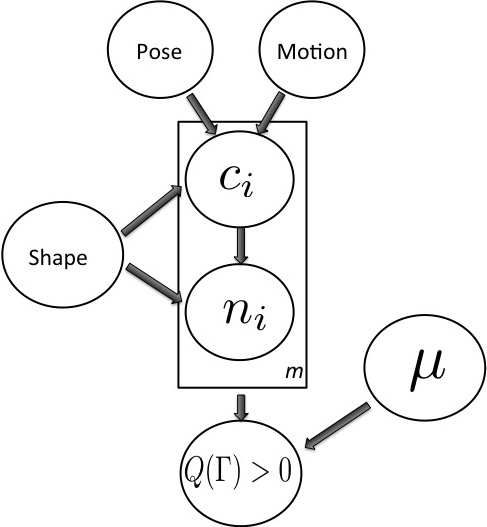
\includegraphics[width = 6cm, height = 6cm]{figures/Slide8.jpg}
\caption{A graphical model that illustrates the relationship between the different types of uncertainty in an object. Center of Mass uncertainty is dependent on the pose and shape of the object, however friction coefficient is independent of all other types. }
\vspace*{-10pt}
\label{fig:graphical_model}
\end{figure}


\begin{figure}[ht!]
\centering
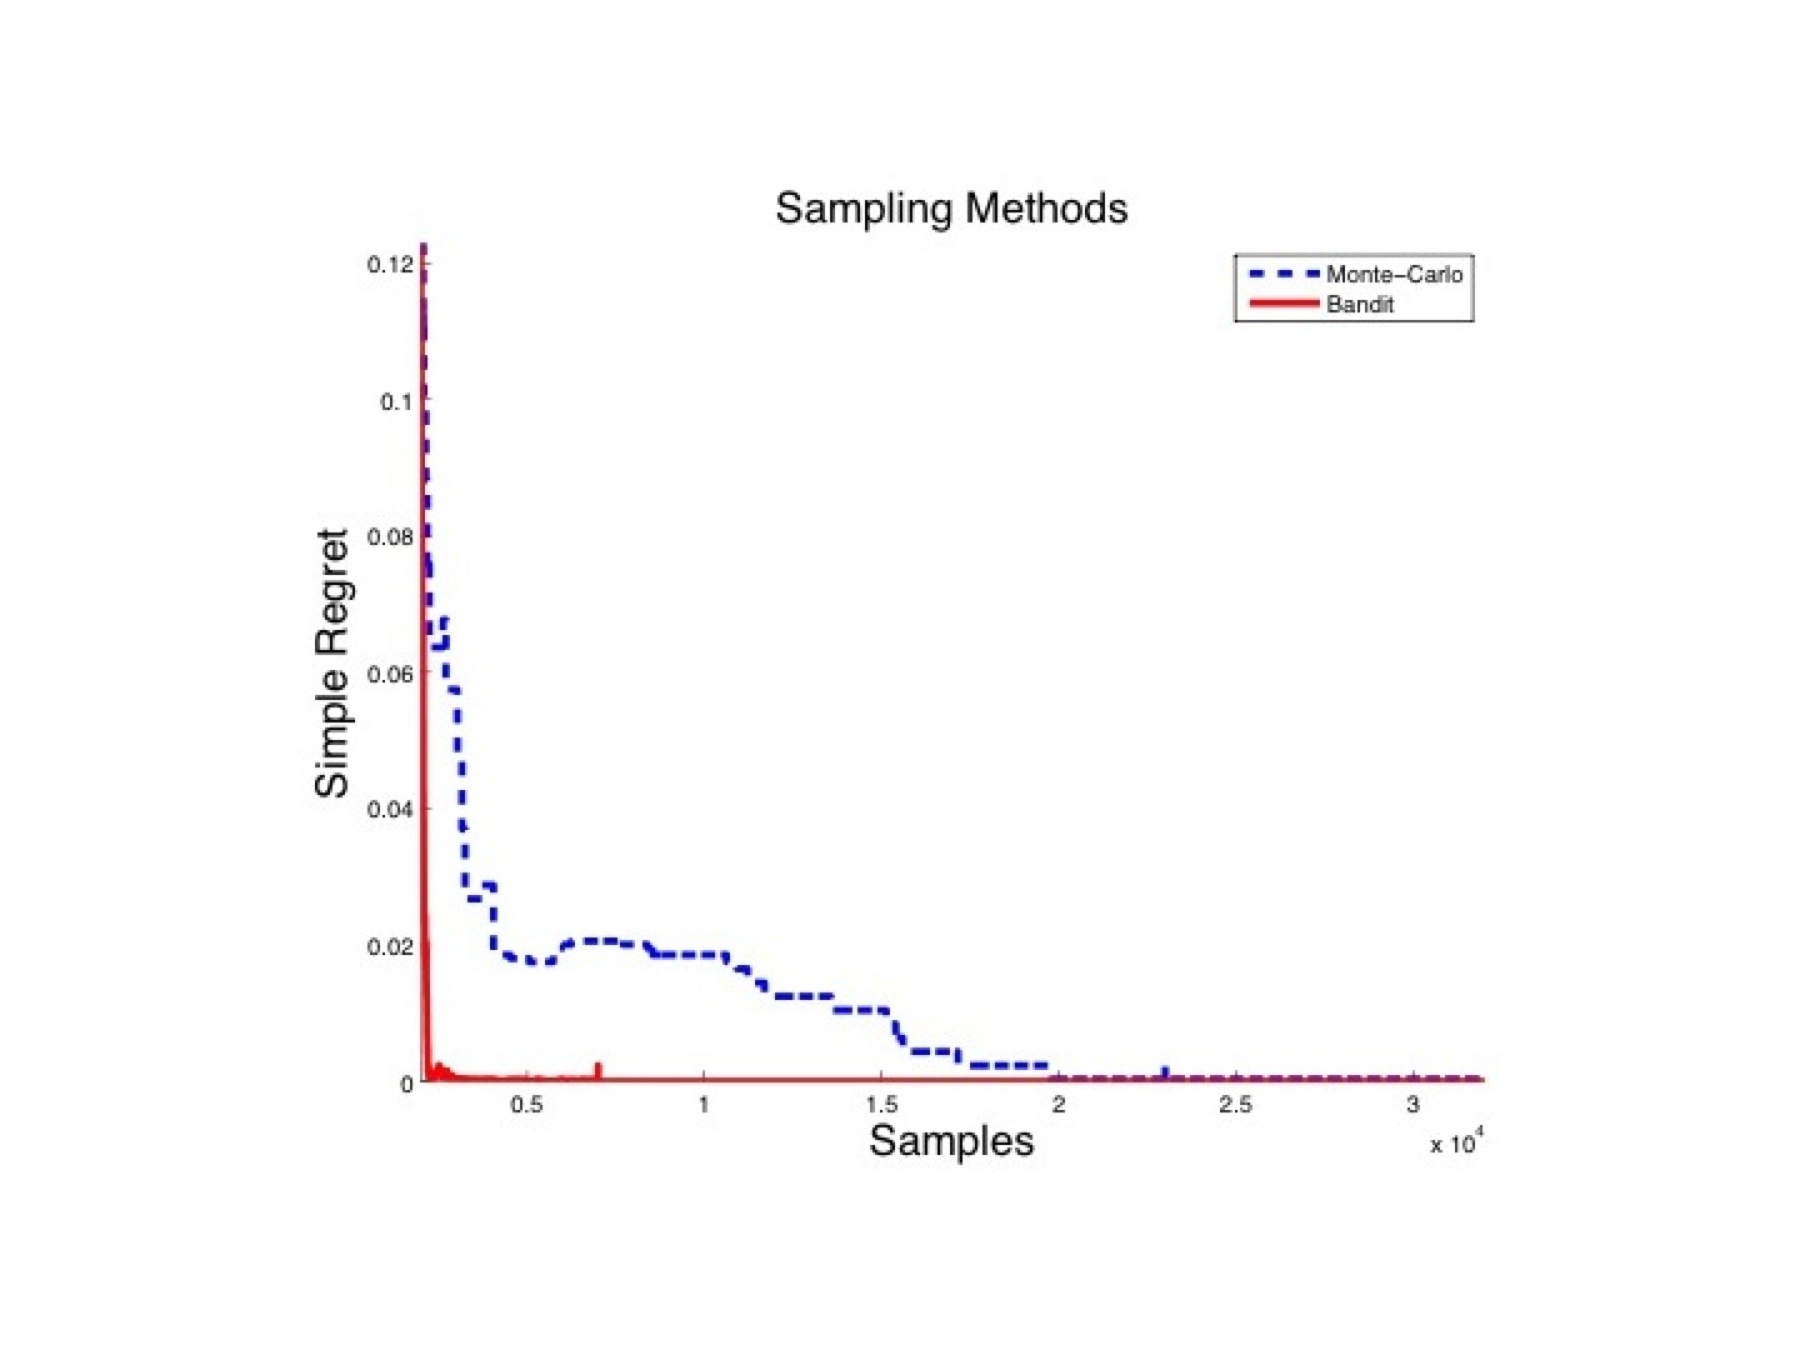
\includegraphics[width = 6cm, height = 4cm]{figures/Slide01.jpg}
\caption{Illustration of a grasp plan $\Gamma$ composed of two lines of action, $\gamma_1(t)$ and $\gamma_2(t)$}
\vspace*{-10pt}
\label{fig:line_of_action}
\end{figure}


\subsection{Problem Definition}

We assume we are given a 2-D workspace $\mathcal{W}$ with an unknown object represented as a trained GPIS model, described in Section \ref{sec:GP}, and set of possible grasp plans $G$ which are generated either randomly or with a heuristic as in \cite{mahler2015gp}.
We are interested in determining Eq. \ref{eq:problem_def} with respect to a chosen grasp metric Q. 

\vspace{-2ex}
\begin{align}\label{eq:problem_def}
\Gamma^* \in \underset{\Gamma \in G}{\mbox{argmax}} P(Q(\Gamma)>0)
\end{align}

\section{Distributions on Grasp Parameters}
\label{sec:distgrasp}
 
 To sample from $p(Q(\Gamma)>0)$, we need to sample from the distributions associated with a line of action $p(\textbf{n}_i,\textbf{c}_i|\gamma_i(t),\Delta,\theta, \rho)$. Using Bayes rule and our graphical model we can rewrite this as 
 
 \vspace{-2ex}
 \begin{align*}
 &p(\textbf{n}_i,\textbf{c}_i |\gamma_i(t),\theta,\Delta,\rho)=\\
 &p(\textbf{n}_i|\textbf{c}_i,\theta)p(\textbf{c}_i|\gamma_i(t),\theta,\rho,\Delta)
 \end{align*}
 
 In section \ref{sec:contact}, we look at how to draw shape sample from a GPIS model, which is used to compute $p(\textbf{c}_i|\gamma_i(t),\theta,\rho,\Delta)$ along with the other sampled distribution on pose ($\Delta$) and motion ($\rho$). Then in section \ref{sec:normals}, we look at how to sample from $p(\textbf{n}_i|\textbf{c}_i,\theta)$ and present a novel visualization technique for the distribution on surface normals. Lastly in section \ref{sec:mass}, we show a way to calculate the expected center of mass assuming a uniform mass distribution. 
 .
\subsection{Distribution on Surface Normals}\label{sec:normals} 
Using Eq. \ref{eq:mean_gradient} and Eq. \ref{eq:cov_gradient}, we can compute the mean of the gradient $ \mu_{\nabla}(x)$ and the covariance of the gradient $\Sigma_{\nabla}(x)$ respectively. Thus we can compute the distribution around the surface normal for a given point in $\mathcal{W}$. We can now write 

One interesting effect of this technique is that we can now marginalize out the line of action model and visual what the surface normal distribution is along a given line of action. To our knowledge this is the first attempt to visual surface normals along a grasp plan. Marginalization can be performed as follows:

\vspace{-2ex}
\begin{equation}
    p(\textbf{n}_i ) = \int_a^b   p\big(\textbf{n}_i = \textbf{v} | \textbf{c}_i = \gamma(t) \big)p\big(\textbf{c}_i = \gamma(t)\big) dt \label{eq:normal_dist}
\end{equation}

Grasp metrics such as  Ferrari-Canny require $\textbf{n}_i$ be normalized, or, equivalently, a member of the sphere $\mathcal{S}^{d-1}$ \cite{ferrari1992}. To account for this we densely sample from the  distribution $p \big(\textbf{n}_i ) \big)$  and project onto $\mathcal{S}^{d-1}$.  In Fig.\ref{fig:GraspDist}, we visualize the distribution on $\textbf{n}_i$ calculated for a given GPIS and approach line of action.


\subsection{Expected Center of Mass}\label{sec:mass} 

We recall the quantity $P(sd(x) < 0) = \int_{-\infty}^{0} p(sd(x) =  s \ | \ \mu(x),\Sigma(x)) ds$ is equal to the probability that $x$ is interior to the surface under the current observations.
We assume that the object has uniform mass density and then $P(sd(x) < 0)$ is the expected mass density at $x$.
Then we can find the expected center of mass as:

\label{eq:mass}
\begin{equation}
  \bar{z} 
  =
  \frac
    {\int_{\mathcal{W}}x P(sd(x)<0) dx}
    {\int_{\mathcal{W}}  P(sd(x)<0) dx}
\end{equation}

which can be approximated by sampling $\mathcal{W}$ in a grid and approximating the spatial integral by a sum. Since this operation involves the entire SDF, one would want to use a low resolution grid for computational efficiency. We show the computed density and calculated expected center of mass for a marker in Fig. \ref{fig:GPIS_MASS}.


\begin{figure}[ht!]
\centering
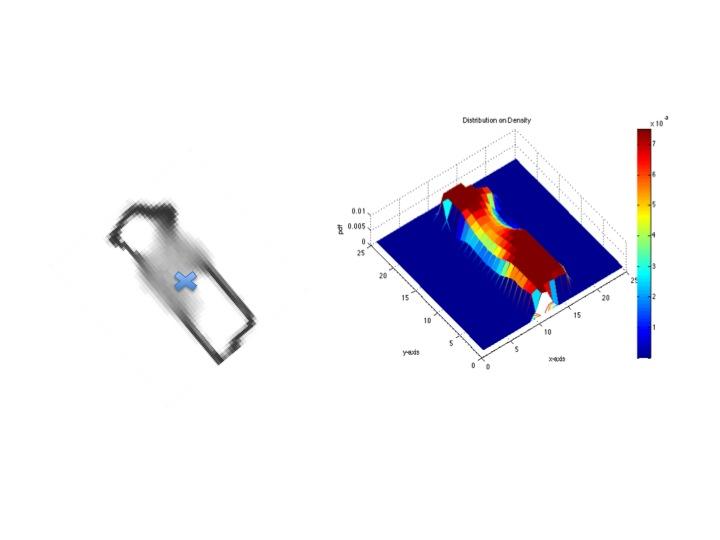
\includegraphics[scale = 0.3]{figures/Slide06.jpg}
\caption{ \footnotesize Left: A surface with GPIS construction and expected center of mass (black X)
Right: The distribution on the density of each point assuming uniform density}
\vspace*{-10pt}
\label{fig:GPIS_MASS}
\end{figure}


\section{Multi-Armed Bandits for Grasp Selection}
While a standard approach to solving the problem in Eq. \ref{eq:problem_def} would be to perform Monte-Carlo integration on each $\Gamma_i$ and compute the expected grasp quality, we propose treating the problem as a multi-armed bandit model and forming a policy for selecting which grasp to sample. 
In our setting, we have a probabilistic shape representation and would like to evaluate many potential grasps on that shape model.
Motivated by limited computational resources we are interested in how to intelligently allocate sampling resources to efficiently find the best grasp plan $\Gamma^*$.
Here each arm corresponds to a different grasp plan and pulling the arm is sampling from the graphical model in Fig. \ref{fig:graphical_model} and evaluating the arm's grasp plan on the sample.
The reward for pulling an arm is 1 if the grasp is in force closure on the sample and 0 if the grasp is not in force closure. 

We can now model the distribution on rewards as a Beta-Bernoulli process. Bernoulli distributions are formally the probability $\theta$ that an event has occurred and a Beta distribution is the conjugate prior on the probability of theta or $p(\theta)$. Beta distributions are specified by shape parameters $\alpha$ and $\beta$, to update the prior Beta distribution one simply adds the count of observed successes of the event to $\alpha$ and the count of the observed failures to $\beta$. The default $\alpha =1 $ and $\beta =1$ corresponds to a uniform distribution on $\theta$. 

Since, we have framed the method as a Beta-Bernoulli problem we can use the methods in Sec.\ref{sec:algorithms} and obtain guarantees in the convergence properties of regret and overall performance of our policy for grasp allocation. 





\section{Calculating the Probability of Force Closure}
Given a proposed grasp plan $\Gamma$ , we draw samples from the shape distribution $P (\theta )$, the distribution on center of pose $P (\Delta)$, distribution on motion $p(\rho)$ and the distribution on friction coefficient $P (\mu)$. The distribution on force closure can then be estimated as Beta- Bernoulli Process with shape parameters $\alpha$ and $\beta$. Thus, we can write the expected probability of force closure as follows


\vspace{-2ex}
\begin{align}\label{eq:shape_sampling}
P(Q(\Gamma|\theta,\mu,\Delta,\rho) > 0) = \frac{\alpha}{\alpha + \beta}
\end{align}

Where $Q(\Gamma|S,\mu,z)$ is the grasp quality that is computed on a shape sample drawn from $p(S)$,$p(\Delta)$,$p(\rho)$ and $p(\mu)$. To compute this we intersect the zero crossing of the level set with the propose grasp plan $\Gamma$ and determine the parameters $g$, this has been the approach taken in previous work  \cite{kehoe2012estimating}, \cite{kehoe2012toward},  \cite{christopoulos2007handling}. Whats interesting in the context of a BMAB problem our complicated graphical model in Fig. \ref{fig:graphical_model}, can now be replaced by \ref{fig:beta_model} and we only need to estimate $\alpha$ and $\beta$ to determine grasp quality. It is this intuition that helps explain the performance of the BMAB algorithm. 

\begin{figure}[ht!]
\centering
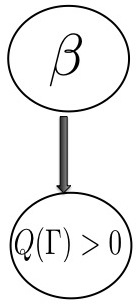
\includegraphics[width = 2cm, height = 4cm]{figures/Slide9.jpg}
\caption{A graphical model that illustrates the relationship between the Bernoulli distribution of the probability force closure and its conjugate prior Beta distribution that has two shape parameters $\alpha$ and $\beta$ }
\vspace*{-10pt}
\label{fig:beta_model}
\end{figure}


\section{Experiments}
For the experiments below we used common household objects.  The objects used can be found at \url{http://rll.berkeley.edu/grasping/} We manually created a 25 x 25 grid, by tracing a point cloud of the object on a table taken with a Primesense Carmine depth sensor. To accompany the SDF, we created an occupancy map, which holds 1 if the point cloud was observed and 0 if it was not observed, and a measurement noise map, which holds the variance 0-mean noise added to the SDF values. The parameters of the GPIS were selected using maximum likelihood on a held-out set of validation shapes. Our visualization technique follows the approach of \cite{mahler2015opt} and consisted of drawing many shape samples from the distribution and blurring accordingly to a histogram equalization scheme. 

We did experiments for the case of two hard contacts in 2-D, however our methods are not limited to this implementation. We drew random lines of actions $\gamma_1(t)$ and $\gamma_2(t)$ by sampling around a circle with radius $\sqrt{2}n$ and sampling the circles origin, then projecting onto the largest inscribing circle in the workspace. 





\subsection{Multi-Armed Bandit Experiments}
\todo{Running experiments over break, going to fill this in as results come in}
We consider the problem of selecting the best grasp plan, $\Gamma^*$ out of a set $G$. For our experiments we look at selecting the best grasp out of a size of $|G| = 1000$. In Fig. \ref{fig:simple_regret}, we plotted the simple regret averaged over 100 of the shapes in our data set and compare the different methods (UCB, Thompson, Gittins and the naive random allocation). We initialize both the Monte-Carlo and bandit technique by sampling each grasp 1 time. We draw samples from our calculated distributions $p(g)$.  Interestingly, Gittins and Thompson converge much faster than random and UCB. In Fig. \ref{fig:pulls_per_grasp}, you can see that Gittins and Thompson allocate grasp samples to only the grasps of high quality, thus it is quickly able to ignore the low quality grasps. UCB takes a more conservative approach to sample allocation, which leads to poor performance in the best arm identification problem \cite{bubeck2009pure}.



\begin{figure*}[ht!]
\centering
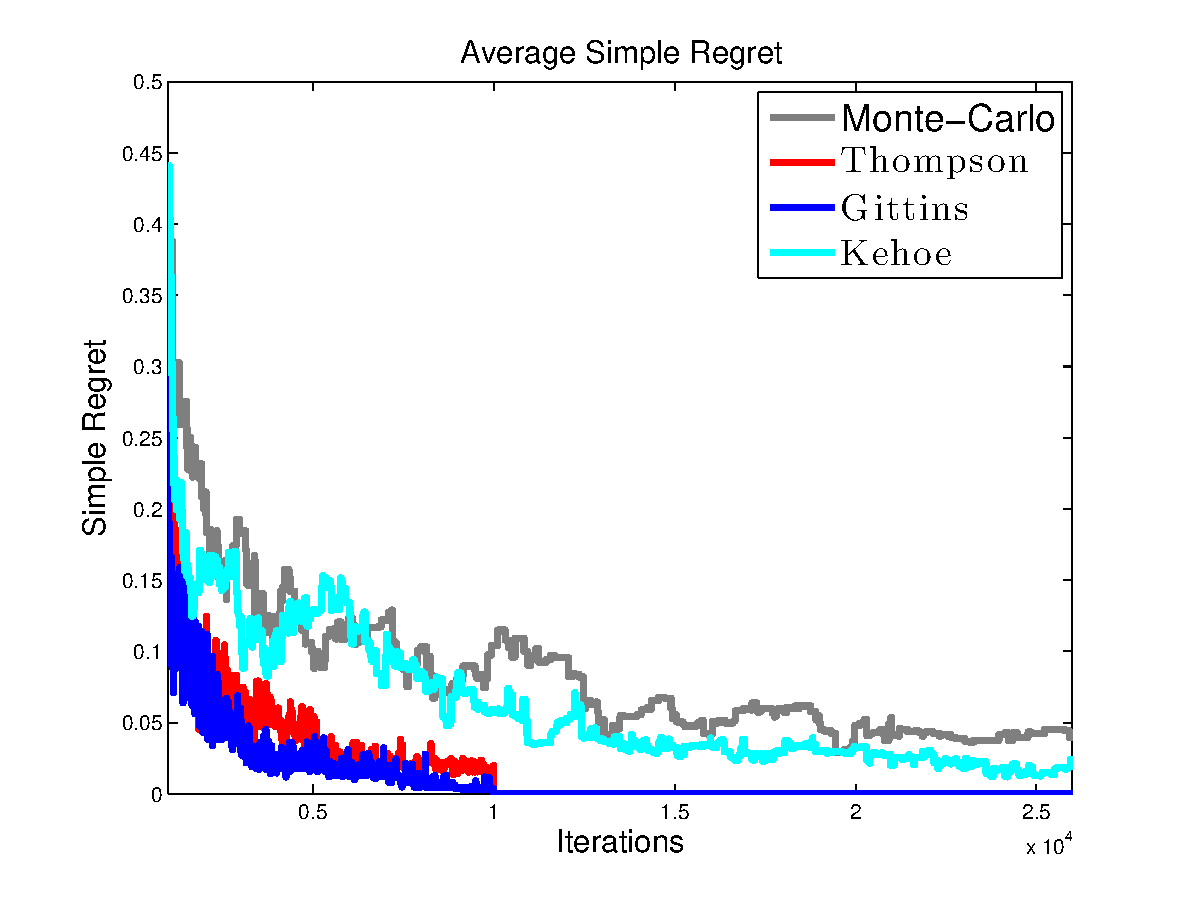
\includegraphics[width = 16.5cm, height = 9cm]{matlab_figures/simple_regret.eps}
\caption{ \footnotesize Comparison of Simple Regret convergence for the four sequential decision methods (Random, UCB, Thompson, Gittins). Graph is averaged over 100 shapes from the Brown Sillohoute Dataset \cite{brown} with a set $|G|=1000$ for each shape. As you can see the Thompson and Gittins method converge almost a magnitude faster than random allocation. UCB does poorly on simple regret which is expected \cite{best_arm}}
\vspace*{-10pt}
\label{fig:simple_regret}
\end{figure*}


\begin{figure*}[ht!]
\centering
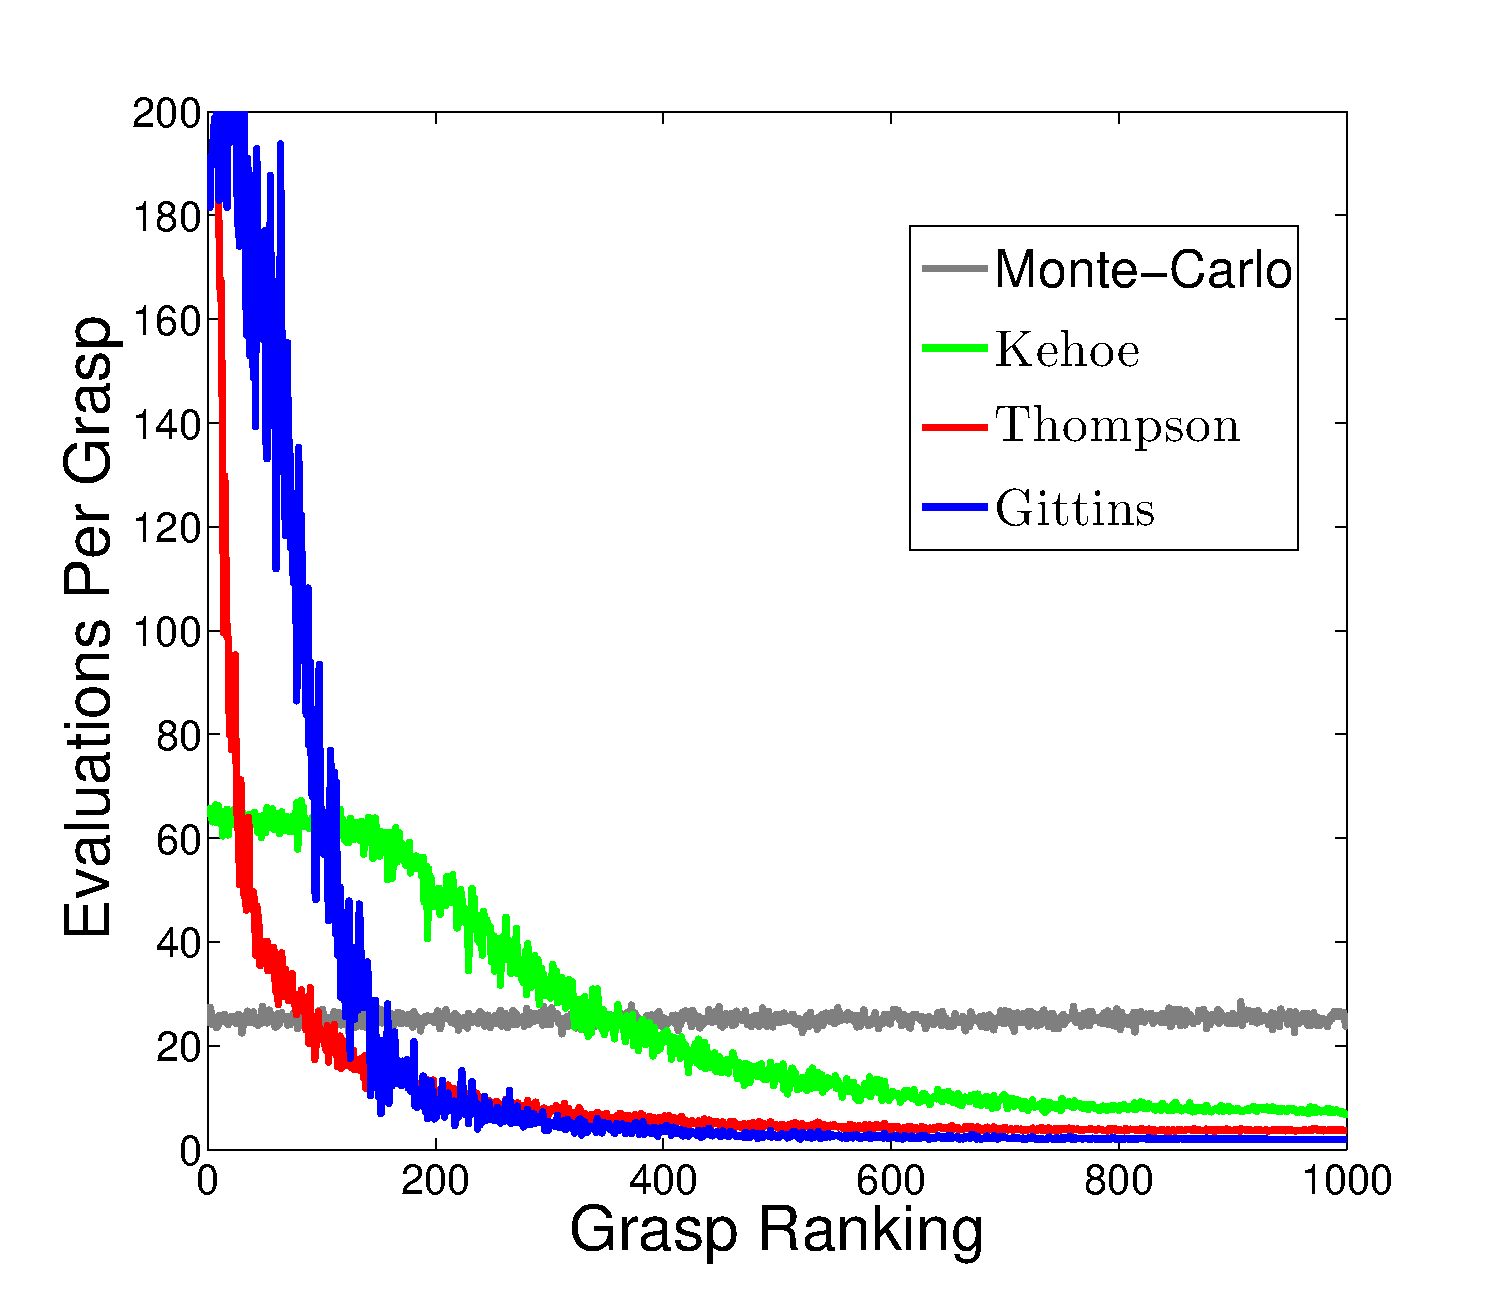
\includegraphics[width = 16.5cm, height = 9cm]{matlab_figures/pulls_per_grasp.eps}
\caption{ \footnotesize Comparison of sample per grasp for the four sequential decision methods (Random, UCB, Thompson, Gittins). Graph is averaged over 100 shapes from the Brown Silhouette Dataset \cite{brown} with a set $|G|=1000$ for each shape. The best grasps are ranked 1 and worst are 1000.  As you can see the Thompson and Gittins method have a tendency to pull grasps with high ranking, while UCB has a more conservative policy \cite{best_arm}}
\vspace*{-10pt}
\label{fig:pulls_per_grasp}
\end{figure*}


\subsection{Sampling from Grasps vs. Shape}
We first tested 1000 grasp plans and sampled each one 5000 times  and measured the RMS error between converged expected grasp plan qualities for sampling shape Eq. \ref{eq:shape_sampling} vs. grasps  Eq. \ref{eq:grasp_sampling} was 0.004. After confirming the distributions converged close to the same value, we show the computational complexity in Fig. \ref{fig:speed_dif} of the two methods for evaluating 100 grasps on an $n \times n$ grid. 



\begin{figure}[ht!]
\centering
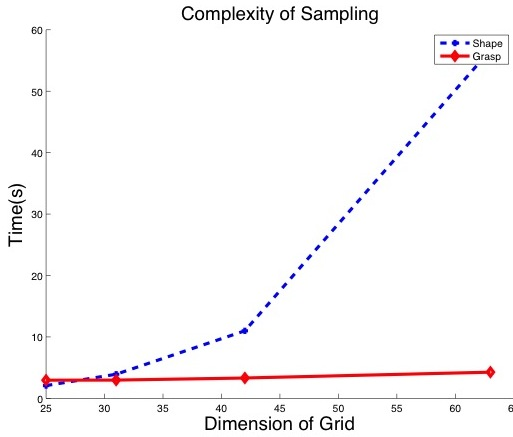
\includegraphics[width=5.7cm,height=6cm]{figures/Slide12.jpg}
\caption{ \footnotesize Time it took to sample from 100 grasp distributions for a given resulution of the workspace. Blue line is sampling from $p(sd(\mathcal{R}))$ or shapes and Red is sampling from $p(g)$ or the calculated distribution on grasps. As you can see sampling from the calculated distributions scales much better. }
\vspace*{-10pt}
\label{fig:speed_dif}
\end{figure}

\section{Limitations} 

Our budgeted multi-armed bandit approach appears promising, but we still do not know how well it will perform on 3D shapes and large scale grids. Future work will be building an efficient construction of GPIS to scale to 3D and test the bandit method there. While we have seen the bandit method always converge to the correct value in our experiments, our method only has a statistical guarantee of doing so. A non-optimal grasp plan could be found, albeit with a low probability. 

Sampling from our distribution $p(g)$ over $p(S)$ yields a reduction in computationally complexity, but only if the number of grasps one wants to evaluate remains small relative to $n^3$, techniques to ensure this could be to find locally optimal potential grasps using optimization approaches \cite{mahler2015opt}. 

An additional problem is that we only have an expected center of mass and not a distribution on the center of mass. This might prove to be to expensive to compute, however recent work by Panahi et al. showed a way to bound the center of mass for convex parts. Extension of his work to implicit surfaces could be of possible interest \cite{panahi2014bounding}.  When using the shape sampling approach on the GPIS instead of sampling along the grasp plan trajectory, the center of mass is easy to compute on a sampled shape, so this is a limitation of our sampling method.

\section{Conclusion}
Assessing grasp quality under shape uncertainty is computationally expensive as it often requires repeated evaluations of the grasp metric over many random samples.
In this work, we proposed a multi-armed bandit approach to efficiently identify high-quality grasps under shape uncertainty. 
A key insight from our work is that uniformly allocating samples to grasps is inefficient, and
 we found that the Successive Elimination multi-armed bandit approach prioritizes evaluation of high-quality grasps while quickly pruning-out obviously poor grasps.
A pre-requisite for applying a bandit approach is to formulate an efficient representation of how shape uncertainty affects grasp parameters and thus grasp quality.
We modeled uncertainty with Gaussian process implicit surfaces (GPIS) and derived the distribution of grasp parameters when a nominal grasp is applied to the GPIS.
As a result, we were able to more efficiently sample from a distribution of grasps executions rather than the shape; leading to a complexity improvement of $n^3$ in the resolution of the discretization $n$.
We evaluated this theoretical model on a dataset of common objects and confirmed that: (1) the bandits approach always converged to the best grasp in the candidate set, (2) it converges on average an order of magnitude faster than a uniform sampling approach in our experiments, and (3) sampling from the grasp contacts is 12x faster than sampling from shapes for a 64x64 grid.



\section{Future Work}
Our results are promising and they suggest many avenues of future work. By utilizing the BMAB model, we can encode uncertainty in the grasp parameters and then leverage the existing algorithms to efficiently find the best grasp. 

In principle, our method can be applied to other representations of shape uncertainty such as perturbations on polygonal vertices \cite{kehoe2012estimating} or splines \cite{christopoulos2007handling}.
It can further be applied to other grasp quality metrics or simulation based evaluation methods \cite{73}. 

Future work will also consider applying BMAB approach to grasp planners like GraspIt! \cite{miller2004graspit} to see if our method can handle uncertainty while working under the time constraints needed for most real time applications. We currently have only tested one bandit algorithm, successive elimination. While our results are promising, it remains to be seen how well it deals with the increased complexity of 3D models over 2D models and larger scale experiments. However, the BMAB model has a large amount of literature to draw from as we encounter new and more challenging problems \cite{bergemann2006bandit}.

\bibliographystyle{IEEEtranS}
\bibliography{references}


\section{Appendix} \label{sec:Appendix}
 In order to solve our problem definition, we must evaluate $P(Q(\Gamma)>0)$ for a given grasp plan $\Gamma$. We will first discuss how the GPIS is constructed, then which grasp metric $Q$ we chose and lastly proceed into evaluating $P(Q(\Gamma)>0)$ efficiently. 


\subsection{Gaussian Process (GP) Background}\label{sec:GP}
We refer the reader to \cite{mahler2015opt} for a more detailed explanation of the GP construction, which we summarize here.  Given the training data $\mD = \{\mX, \by\}$ and covariance function $k(\cdot,\cdot)$, the posterior density $p(sd_*|\bx_*,\mD)$, or the distribution on signed distance field, at a test point $\bx_{*}$ is shown to be \cite{rasmussen2010gaussian}:
\begin{align*}
	p(sd_*|\bx_*,\mD) &\sim \mN\big(\mu(\bx_*), \Sigma(\bx_*)\big) \\
	\mu(\bx_*) &= k(\mX,\bx_*)^{\intercal}(K + \sigma^2I)^{-1}\by \\
	\Sigma(\bx_*) &= k(\bx_*,\bx_*)-k(\mX,\bx_*)^{\intercal}(K+\sigma^2I)^{-1}k(\mX,\bx_*)\big) 
\end{align*}
where $K \in \mathbb{R}^{l \times l}$ is a matrix with entries $K_{ij} = k(\bx_i,\bx_j)$ and $k(\mX,\bx_*) = [k(\bx_1,\bx_*),\ldots,k(\bx_l,\bx_*)]^{\intercal}$. 
This derivation can also be used to predict the mean and variance of the function gradient by extending the kernel matrices using the identities \cite{solak2003derivative}:

\vspace{-2ex}
\begin{align}
	\text{cov}\left(sd(\bx_i), sd(\bx_j) \right) &=  k(\bx_i, \bx_j) \\
	\text{cov}\left(\frac{\partial sd (\bx_i)}{\partial x_k}, sd(\bx_j) \right) &= \frac{\partial}{\partial x_k} k(\bx_i, \bx_j) \label{eq:mean_gradient}\\
	\text{cov}\left(\frac{\partial sd (\bx_i)}{\partial x_k}, \frac{\partial sd (\bx_j)}{\partial x_l} \right) &= \frac{\partial^2}{\partial x_k \partial x_l} k(\bx_i, \bx_j)\label{eq:cov_gradient}
\end{align}


For our kernel choice we decided to use the square exponential kernel, similar to \cite{dragiev2011}. Other kernels relevant to GPIS are the thin-plate splines kernel and the Matern kernel \cite{williams2007}. 


We construct a GPIS by learning a Gaussian process to fit measurements of a signed distance field of an unknown object.  Precisely, $x_i \in \mathbb{R}^2$ in 2D and $x_i \in \mathbb{R}^3$ in 3D, and $y_i \in \mathbb{R}$ is a noisy signed distance measurement to the unknown object at $x_i$.



\subsection{Sampling Shape from GPIS Distribution }
To compute the above distribution we must draw samples from $p(\theta)$. In order to draw shape samples from a GPIS, one needs to sample from signed distance function, $sd$, over the joint on all points in the workspace $\mathcal{W}$ or $p(sd(\mathcal{W}))$. Since this is a GPIS, we know the following 

\vspace{-2ex}
\begin{align}\label{eq:joint_shape}
p(S) = p(sd(\mathcal{W})) \sim N(\mu(\mathcal{W}),\Sigma(\mathcal{W}))
\end{align}

Thus if the workspace is an $n \times n$ grid, the joint distribution is an  $n^2$ multi-variate Gaussian, due to $sd:\mathbb{R}^2 \rightarrow \mathbb{R}$.  Shape samples drawn from the distribution appear in Fig. \ref{fig:shape_samples}.


\begin{figure}[ht!]
\centering
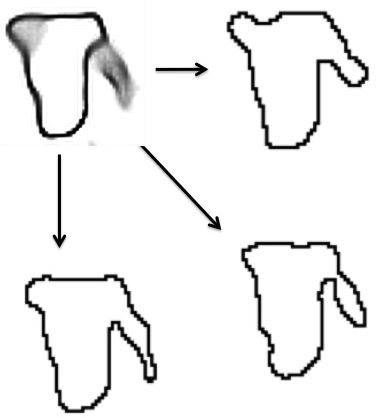
\includegraphics[width = 7.5cm, height= 6cm ]{figures/Slide13.jpg}
\caption{Shape samples drawn from Eq. \ref{eq:joint_shape} on the object in the upper left corner. Given a shape sample we highlight the zero-crossing of the level set in black}
\vspace*{-10pt}
\label{fig:shape_samples}
\end{figure}



\end{document}
